% ==========================================================================
% SLIDE 9: What goes with price per sqft?
% Pauses: click 1 the title (the question); click 2 the intro line and the correlation chart; click 3 the orange headline, the sentence and the grey comment.
% ==========================================================================
\def\secc{kcoral}\def\secct{white}
\begin{frame}[t]{What goes with price per sqft?}
\leavevmode
\atfrom{2}{0.8}{1.4}{14.4}{%
\centering{\normalsize\itshape\color{knavy}Each bar: how a column moves with the price per sqft, in the 18 lower-priced zipcodes}
}
\atfrom{2}{1.5}{2.05}{13}{%
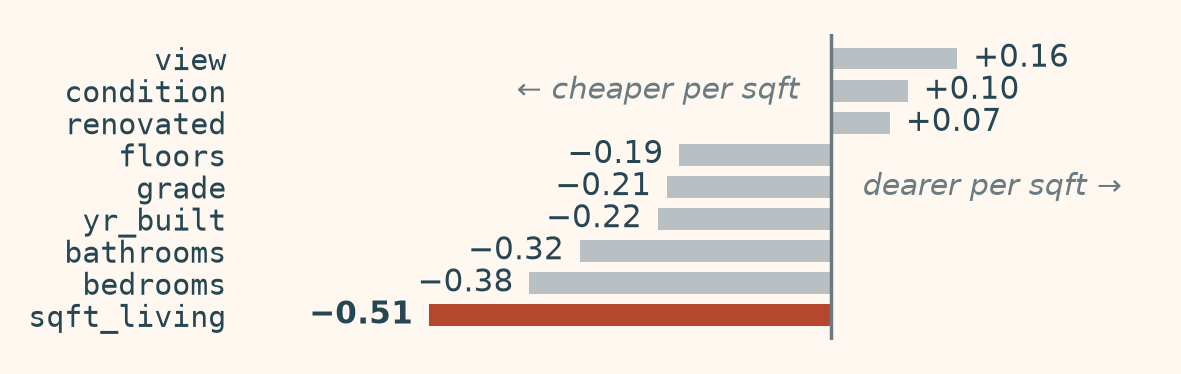
\includegraphics[width=13.00cm]{images/pres_corr.png}
}
\atfrom{3}{0.5}{6.25}{15}{%
\knote{kcoral}{15.00cm}{The bigger the house, the cheaper each sqft}{Big houses cost \textbf{34\%} less per sqft: \$208 under 1,200 sqft, \$138 over 2,500.}
}
\atfrom{3}{0.5}{7.75}{15}{%
{\small\color{knavy!75}Renovating or splitting needs more data.}
}

\end{frame}
